\newpage
\section{Data-driven Character Animation}
使用一些方式连接已有的动作数据.

\subsection{Motion Capture}

\begin{itemize}
    \item Keyframe Animation: 一般用的都是关键帧技术. 把关键帧画出来, 然后用下游方法将其补为动画. 
    \item Motion Capture: vtuber 属于这个 $\left(\enspace{}^{\circ}\;\forall\;{}_{\circ}\enspace\right)$
\end{itemize}

\subsubsection{The History of Mocap}

\begin{itemize}
    \item using photography
    \item Rotoscoping (转描)
    \item Modern Mocap System: 重建动作传感器所给的信息
    \begin{itemize}
        \item Exoskeleton
        \item Inertial Measurement Unit(惯性测量单元, 三加速度计, 三角速度计): 但会有传感器的漂移. 
        \item Optical Mocap: 仅仅是采集标记点, 后期需要区分标记点, 标记点甚至会丢失, 需要手动去补.
        \item Markerless Mocap with Multiple Cameras: 标记点有体积, 其实不太好. 所以就想要无标记点的方法. 
        \subitem 比如用视觉的方法去识别肢体. 
        \subitem 用深度摄像头, RGBD.
    \end{itemize}
    \item Motion Estimation 
    \begin{itemize}
        \item with Monocular Videos: 单视角的信息不全, 会有奇异性. 需要更多的先验. 不算动捕, 只能叫估计.
        \item with Sparse Sensor
    \end{itemize}
\end{itemize}


\subsection{Motion Synthesis}


\begin{figure}[!htb]
    \centering
    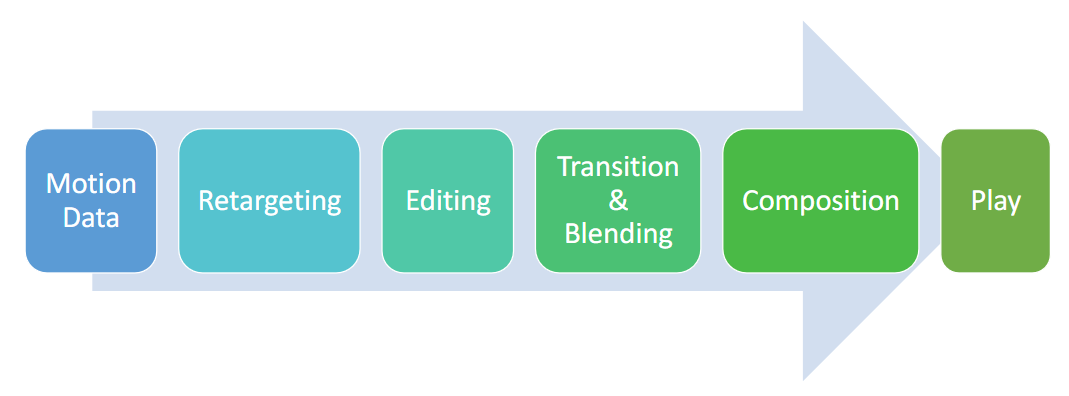
\includegraphics[width=0.88\linewidth]{pic/1055/Using Motion Data}
    \caption{Using Motion Data}
\end{figure}


\subsubsection{Motion Retargeting}
骨骼关节数会不一样, 所以需要用重定向.

如果重定向不好会有: 浮空, 滑步, 穿模等问题. 目前只能手动处理.

A possible retargeting pipeline:
\begin{enumerate}
    \item 映射关键名
    \item 调整尺度
    \item 处理 t pose 的区别. 比如新的节点
    \item 用 ik 处理浮空, 脚打滑等问题
\end{enumerate}

IK Rig: 给关键关节位置, 然后求解 IK, 再得到全部动作.

\subsubsection{Motion Transition}
组合不同的动作

\begin{figure}[!htb]
    \centering
    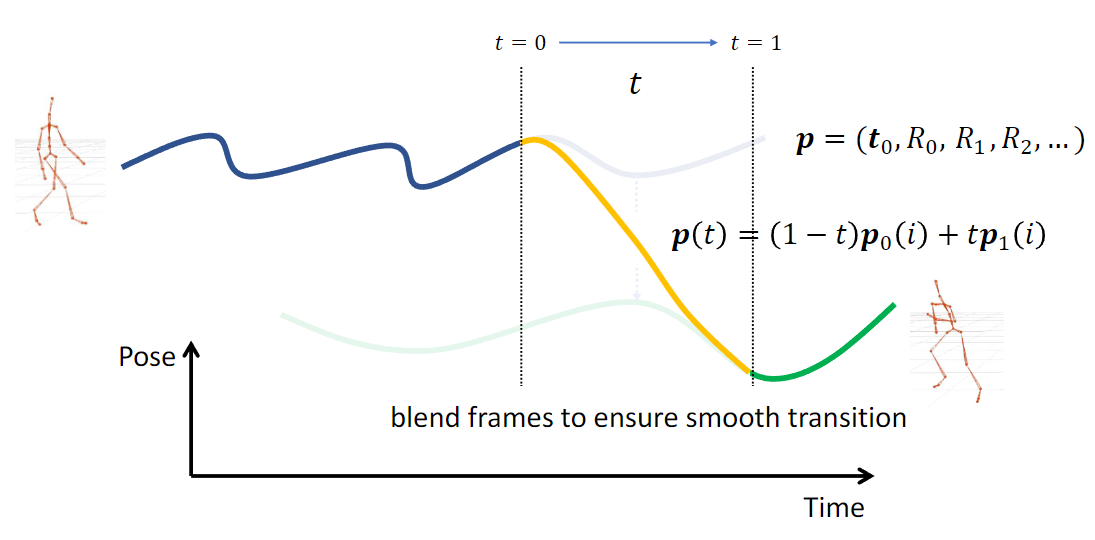
\includegraphics[width=0.88\linewidth]{pic/1055/Motion Transition}
    \caption{Motion Transition}
\end{figure}

切换动作时需要进行平滑操作:
\begin{enumerate}
    \item  取若干帧作插值. 但只是链接地平滑, 不能解决打滑之类的问题. 
    \item 所以还需要对齐. 
\end{enumerate}

\paragraph{Facing Frame} 源点是跟关节在地面的投影. $z$ 轴($y$-up)指向角色朝向(面向方向, 速度方向之类的). 坐标轴定义: 
\begin{align*}
    R &= \theta \bm e_y\\
    \bm t&= (t_x, 0, t_z)
\end{align*}

希望能将根关节旋转分解 $R_0=R_yR_{xz}$, 然后得到 $R_y$

\begin{figure}[!htb]
    \centering
    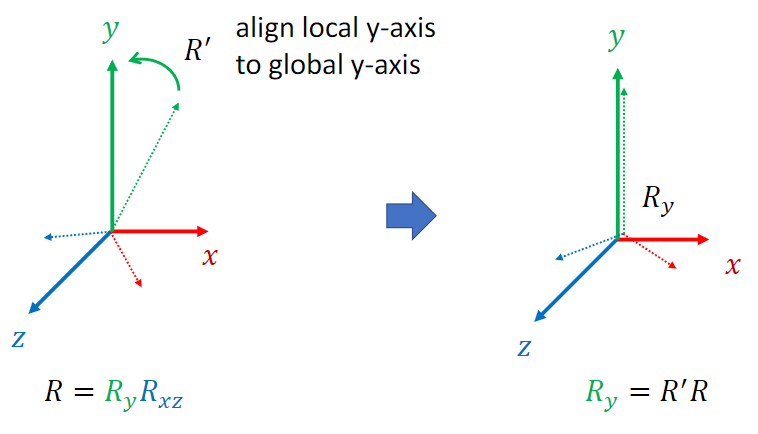
\includegraphics[width=0.618\linewidth]{pic/1055/Rotation Decomposition}
    \caption{Rotation Decomposition}
\end{figure}

然后根据这个对齐两个动作. 

\paragraph{Path Fitting} 有一种可能是没有根关节全局位置, 只有旋转. 一般是游戏里的动作, 这样可以方便让其跟着轨迹走. 

\subsection{Motion}
\subsubsection{Motion Composition}
根据动作生成新的动作. 

\subsubsection{Motion Graphs}
本质上是个状态机. 

\begin{figure}[!htb]
    \centering
    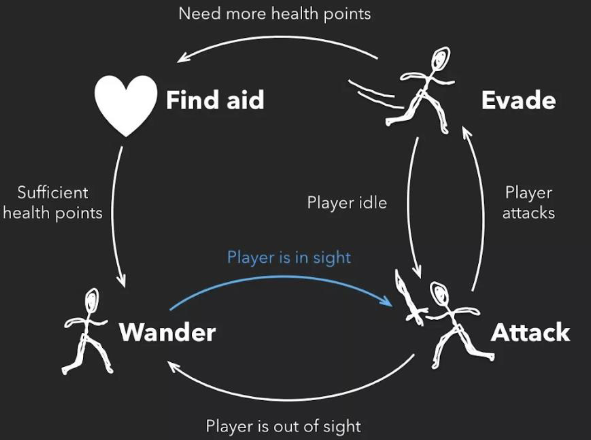
\includegraphics[width=0.618\linewidth]{pic/1055/Motion Graphs}
    \caption{Motion Graphs}
\end{figure}


Segment Motion Data: 主要问题是如果分割运动数据, 如何判定动作可以链接. 
\begin{enumerate}
    \item 定义某种距离, 然后做出 Distance map. 选取图上的局部最小值作为分割点(但效果不好, 还是要手动修)
    \item 然后根据上述信息构造动作图. 
\end{enumerate}

Motion Synthesis using Motion Graphs: 
\begin{itemize}
    \item 结点代表 motion clips
    \item 边代表潜在的 transitions
    \item 当需要时 transitions 被触发, e.g. 用户输入时, clip 结束时
\end{itemize}

\begin{figure}[!htb]
    \centering
    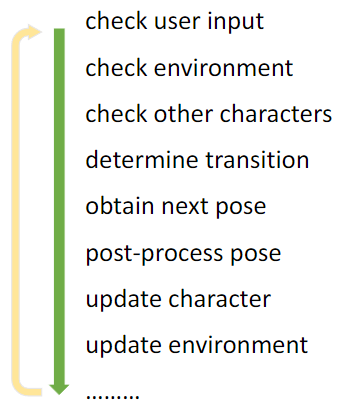
\includegraphics[width=0.42\linewidth]{pic/1055/Interactive Animation Pipeline}
    \caption{Interactive Animation Pipeline}
\end{figure}


\subsubsection{Motion Matching}
对上一帧找下一帧作衔接. 

